\documentclass[12pt,twoside]{article}
\usepackage[ngerman]{babel}
%\usepackage{lmodern}
\usepackage[utf8]{inputenc}
%\usepackage[T1]{fontenc}
%%%%%%%%%%%%%%%%%%%%%%%%%%%%%%%%%%%%%%%%%%%%%%%%%%%%%%%%%%%%%
% Meta informations:
\newcommand{\trauthor}{Louis Kobras}
\newcommand{\trtype}{Proseminararbeit} %{Paper} %{Seminararbeit} %{Proseminararbeit}
\newcommand{\trcourse}{Proseminar: Künstliche Intelligenz}
\newcommand{\trtitle}{Generieren dynamischer Antworten durch Parsing von natürlicher Sprache}
\newcommand{\trmatrikelnummer}{6658699}
\newcommand{\tremail}{4kobras@informatik.uni-hamburg.de}
\newcommand{\trarbeitsbereich}{Knowledge Technology, WTM}
\newcommand{\trdate}{\today}

%%%%%%%%%%%%%%%%%%%%%%%%%%%%%%%%%%%%%%%%%%%%%%%%%%%%%%%%%%%%%
% Bind packages:
\usepackage{acronym}                    % Acronyms
\usepackage{algorithmic}				% Algorithms and Pseudocode
\usepackage{algorithm}					% Algorithms and Pseudocode
\usepackage{amsfonts}                   % AMS Math Packet (Fonts)
\usepackage{amsmath}                    % AMS Math Packet
\usepackage{amssymb}                    % Additional mathematical symbols
\usepackage{amsthm}
\usepackage{booktabs}                   % Nicer tables
%\usepackage[font=small,labelfont=bf]{caption} % Numbered captions for figures
\usepackage{color}                      % Enables defining of colors via \definecolor
\definecolor{uhhRed}{RGB}{254,0,0}		% Official Uni Hamburg Red
\definecolor{uhhGrey}{RGB}{122,122,120} % Official Uni Hamburg Grey
\usepackage{fancybox}                   % Gleichungen einrahmen
\usepackage{fancyhdr}					% Packet for nicer headers
%\usepackage{fancyheadings}             % Nicer numbering of headlines
\usepackage{perpage}					% resets specified settings per page
\MakePerPage{footnote}					% resetting footnote count per page

\usepackage[outer=3.35cm]{geometry} 	% Type area (size, margins...) !!!Release version
%\usepackage[outer=2.5cm]{geometry} 	% Type area (size, margins...) !!!Print version
%\usepackage{geometry} 					% Type area (size, margins...) !!!Proofread version
%\usepackage[outer=3.15cm]{geometry} 	% Type area (size, margins...) !!!Draft version
\geometry{a4paper,body={5.8in,9in}}

% changing font
\usepackage{times}

\usepackage{graphicx}                   % Inclusion of graphics
%\usepackage{latexsym}                  % Special symbols
\usepackage{longtable}					% Allow tables over several parges
\usepackage{listings}                   % Nicer source code listings
\usepackage{multicol}					% Content of a table over several columns
\usepackage{multirow}					% Content of a table over several rows
\usepackage{rotating}					% Alows to rotate text and objects
\usepackage[hang]{subfigure}            % Allows to use multiple (partial) figures in a fig
%\usepackage[font=footnotesize,labelfont=rm]{subfig}	% Pictures in a floating environment
\usepackage{tabularx}					% Tables with fixed width but variable rows
\usepackage{url,xspace,boxedminipage}   % Accurate display of URLs
\usepackage{hyperref}
% listing captions
\usepackage{caption}
% tikz being tikz
\usepackage{tikz}
\usetikzlibrary{arrows,automata}
\usepackage{pgf}
%%%%%%%%%%%%%%%%%%%%%%%%%%%%%%%%%%%%%%%%%%%%%%%%%%%%%%%%%%%%%
% Configurationen:

\hyphenation{whe-ther} 					% Manually use: "\-" in a word: Staats\-ver\-trag

%\lstloadlanguages{C}                   % Set the default language for listings
\DeclareGraphicsExtensions{.pdf,.svg,.jpg,.png,.eps} % first try pdf, then eps, png and jpg
\graphicspath{{./src/}} 								% Path to a folder where all pictures are located
\pagestyle{fancy} 											% Use nicer header and footer

% Redefine the environments for floating objects:
\setcounter{topnumber}{3}
\setcounter{bottomnumber}{2}
\setcounter{totalnumber}{4}
\renewcommand{\topfraction}{0.9} 		%Standard: 0.7
\renewcommand{\bottomfraction}{0.5}		%Standard: 0.3
\renewcommand{\textfraction}{0.1}		%Standard: 0.2
\renewcommand{\floatpagefraction}{0.8} 	%Standard: 0.5

% Tables with a nicer padding:
\renewcommand{\arraystretch}{1.2}
%
%% custom titles for TOC and References
%\renewcommand{\contentsname}{whatever}
%\renewcommand{\refname}{WASD-Force}
%\renewcommand{\bibname}{DSAW-Force}

%%%%%%%%%%%%%%%%%%%%%%%%%%%%
% Additional 'theorem' and 'definition' blocks:
\theoremstyle{plain}
\newtheorem{theorem}{Theorem}[section]
%\newtheorem{theorem}{Satz}[section]		% Wenn in Deutsch geschrieben wird.
%\newtheorem{axiom}{Axiom}[section] 	
%\newtheorem{axiom}{Fakt}[chapter]		% Wenn in Deutsch geschrieben wird.
%Usage:%\begin{axiom}[optional description]%Main part%\end{fakt}

\theoremstyle{definition}
\newtheorem{definition}{Definition}[section]

%Additional types of axioms:
%\newtheorem{lemma}[axiom]{Lemma}
%\newtheorem{observation}[axiom]{Observation}

%Additional types of definitions:
\theoremstyle{remark}
\newtheorem{remark}[definition]{Bemerkung} % Wenn in Deutsch geschrieben wird.
%\newtheorem{remark}[definition]{Remark} 

%%%%%%%%%%%%%%%%%%%%%%%%%%%%
% Provides TODOs within the margin:
\newcommand{\TODO}[1]{\marginpar{\emph{\small{{\bf TODO: } #1}}}}

%%%%%%%%%%%%%%%%%%%%%%%%%%%%
% Abbreviations and mathematical symbols
\newcommand{\modd}{\text{ mod }}
\newcommand{\RS}{\mathbb{R}}
\newcommand{\NS}{\mathbb{N}}
\newcommand{\ZS}{\mathbb{Z}}
\newcommand{\dnormal}{\mathit{N}}
\newcommand{\duniform}{\mathit{U}}

\newcommand{\erdos}{Erd\H{o}s}
\newcommand{\renyi}{-R\'{e}nyi}

%%%%%%%%%%%%%%%%%%%%%%%%%%%
% Source code inclusion
\definecolor{pblue}{rgb}{0.13,0.13,1}
\definecolor{pgreen}{rgb}{0,0.5,0}
\lstset{ %
language=Python,   							% choose the language of the code
basicstyle=\small\ttfamily,  				% the size of the fonts that are used for the code
numbers=left,                   			% where to put the line-numbers
numbersep=5pt,                  			% how far the line-numbers are from the code
backgroundcolor=\color{light-light-gray},   % choose the background color. You must add
frame=lrtb,           						% adds a frame around the code
tabsize=4,          						% sets default tabsize to 2 spaces
captionpos=b,           					% sets the caption-position to bottom
breaklines=true,        					% sets automatic line breaking
xleftmargin=1.5cm,							% space from the left paper edge
commentstyle=\color{pgreen},
keywordstyle=\color{pblue},
literate=%
    {Ö}{{\"O}}1
    {Ä}{{\"A}}1
    {Ü}{{\"U}}1
    {ß}{{\ss}}1
    {ü}{{\"u}}1
    {ä}{{\"a}}1
    {ö}{{\"o}}1
    {~}{{\textasciitilde}}1
}
\renewcommand{\lstlistingname}{Code}
\captionsetup[lstlisting]{font={footnotesize},margin=1.5cm,singlelinecheck=false } % removes "Listing 1: "
\definecolor{light-light-gray}{gray}{0.95}

% decreasing space used above and below figures
\setlength{\belowcaptionskip}{-10pt}
\setlength{\abovecaptionskip}{10pt}


%%%%%%%%%%%%%%%%%%%%%%%%%%%%%%%%%%%%%%%%%%%%%%%%%%%%%%%%%%%%%
% Document:
\begin{document}
\renewcommand{\headheight}{14.5pt}

\fancyhead{}
\fancyhead[LE]{ \slshape \trauthor}
\fancyhead[LO]{}
\fancyhead[RE]{}
\fancyhead[RO]{ \slshape \trtitle}

%%%%%%%%%%%%%%%%%%%%%%%%%%%%
% Cover Header:
\begin{titlepage}
	\begin{flushleft}
		Universit\"at Hamburg\\
		Department Informatik\\
		\trarbeitsbereich\\
	\end{flushleft}
	\vspace{3.5cm}
	\begin{center}
		\huge \trtitle\\
	\end{center}
	\vspace{3.5cm}
	\begin{center}
		\normalsize\trtype\\
		[0.2cm]
		\Large\trcourse\\
		[1.5cm]
		\Large \trauthor\\
		[0.2cm]
		\normalsize Matr.Nr. \trmatrikelnummer\\
		[0.2cm]
		\normalsize\tremail\\
		[1.5cm]
		\Large \trdate
	\end{center}
	\vfill
\end{titlepage}

	%backsite of cover sheet is empty!
\thispagestyle{empty}
\hspace{1cm}
\newpage

%%%%%%%%%%%%%%%%%%%%%%%%%%%%
% Abstract:

% Abstract gives a brief summary of the main points of a paper:
\section*{Abstract}
Seit Jahrzehnten schon beschäftigen sich Forscher damit, den Computer dem Menschen näher zu bringen.
Ein wichtiger Bestandteil dieses Prozesses ist dabei die Sprachverarbeitung.\\
Ziel dieser Arbeit ist, Licht auf den Prozess des Verständnisses eines Computers von natürlicher Sprache zu werfen.\\
Zu diesem Zweck wird der Begriff der natürlichen Sprache in seine Komponenten zerlegt,
die einzelnd analysiert und in dieser Form von nichtkomplexen Automaten verarbeitet werden können.\\
Im Hinblick auf die Entwicklung von Videospielen wird mithilfe der \textit{String}-Klasse von Java, der \textit{RexEx}-Konvention und dem ELIZA-Programm eine Möglichkeit gezeigt, jeden beliebigen Eingabetext zu analysieren und darauf zu reagieren.
% Lists:
\setcounter{tocdepth}{2} 					% depth of the table of contents (for Seminars 2 is recommented)
\tableofcontents
\pagenumbering{arabic}
\clearpage

%%%%%%%%%%%%%%%%%%%%%%%%%%%%
% Content:

% the actual content, usually separated over a number of sections
% each section is assigned a label, in order to be able to put a
% crossreference to it
\section{Einführung}
\label{sec:intro}
	Schon seit etwa achtzig Jahren beschäftigen sich Forscher mit dem Thema der Künstlichen Intelligenz, und nicht weniger Zeit ist in die Theorie der Sprachverarbeitung investiert worden.
	Sprachverarbeitung liegt in zwei Formen vor, die in ihren jeweiligen Anwendungsgebieten für eine erhebliche Steigerung der Effektivität der Nutzer sorgen können: Verarbeitung \textit{gesprochener Sprache} (Speech Recognition) und \textit{Textverarbeitung} (Text Processing).
	Beide Aspekte fallen unter das \textit{Verarbeiten natürlicher Sprache} (Natural Language Processing).
	Diese Arbeit wird sich mit dem Verarbeiten natürlicher Sprache in Textform beschäftigen.\\
	Zwar ist Kommunikation durch Texteingabe nicht so schnell und dynamisch anwendbar wie gesprochene Anweisungen, dennoch aber ist sie ein wichtiger Schritt dorthin.
	Wir werden sehen, wie natürliche Sprache aufgebaut ist, wie sie durch Verwendung von Deterministischen Automaten und Regulären Ausdrücken analysiert werden kann, und wie mit den erhaltenen Informationen verfahren werden kann.
	\subsection{Was bisher geschah: Sprachverarbeitung im Kontext der historischen Artificial Intelligence}
	\label{ssec:history}
	Die Grundsteine für Künstliche Intelligenz wurden 1936 von Turing und darauf aufbauend in den 40ern und 50ern gelegt (McCulloch und Pitts (1943), Chomsky (1956) et. al.).\\
	Ende der 50er Jahre hatten sich daraus zwei parallele Zweige für die Sprachverarbeitung gebildet: Das formale Paradigma und der stochastische Ansatz (\cite{Jur2009}).\\
	Während das formale Paradigma seinen Schwerpunkt auf formale Sprachen und das Parsen von Schlüsselwörtern gelegt hatte, lag der Schwerpunkt des anderen Ansatzes auf der Berechnung der Wahrscheinlichkeit des Auftretens bestimmter Wörter anhand eines umfassenden Lexikons und der Anwendung Bayesscher Methoden auf die einzelnen Zeichen.\\
	Während der stochastische Zweig weitestgehend erhalten blieb, teilte sich der formale Zweig zu Beginn der 70er Jahre in drei Pfade auf.
	Der stochastische Zweig begann, versteckte Markov-Modelle (HMM) bei seiner Analyse zu nutzen.
	Ein Logik-basierender Zweig befasste sich mit der Vereinheitlichung der Struktur von Sprache und nutzte dabei eine sog. \textit{Definite Clause Grammar}, woraus sich später Prolog entwickeln würde.
	Der Zweig, der sich mit natürlicher Sprache befasste, versuchte, Text-Kommandos und Konzepte so umzusetzen, dass Maschinen eine semantische Grundlage mitgegeben werden konnte, auf der die Interpretation aufbauen würde.
	Der Diskurs-Zweig verwendete die Betrachtung von Substrukturen im Diskurs von Sprachen und der Automatisierung von Referenzen.\\
	Die 80er und 90er Jahre beschäftigten sich Wahrscheinlichkeitsmodellen und Modellen, die sich deterministische, endliche Automaten zur Analyse zu Nutzen machten.\\
	Ende des 20. Jahrhunderts hatte sich das Wahrscheinlichkeitsmodell als Standard durchgesetzt. Die Forschung in diesem Feld wurde durch das Aufkommen des Internet und auf kommerzieller Basis durch Entwicklung der Technologie weiter vorangetrieben.
	\subsection{ELIZA als Beispiel für frühe Sprachverarbeitung}
	\label{ssec:eliza}
	ELIZA ist ein frühes Programm zur Sprachverarbeitung (Weizenbaum, 1966).
	Das Programm wendet simples Parsing und Mustererkennung an, um Schlüsselwörter aus einem gegebenen Satz zu extrahieren und darauf aufbauend eine Antwort zu generieren.
	ELIZA arbeitet als Rogativer Psychologe, d.h. man erzählt ihr etwas und sie stellt eine darauf basierende Frage.\\
	Das Programm ist sehr simpel, und ELIZA benötigt fast keine Informationen, um zu funktionieren.
	Durch ihre Arbeitsweise kann sie ein natürliches Gespräch mit einem Psychologen nur durch das Wiederholen von Sätzen in Frageform erfolgreich simulieren.
	Dies tut sie, indem sie mit einem simplen Such-Algorithmus den vom Benutzer eingegebenen Text mit einer Liste von Stichworten vergleicht und anhand derer eine vordefinierte Antwort zurückliefert.
	Zugegebenermaßen ist die Art der Antworten derart gut konstruiert, dass viele der Probanden, die in den 60er Jahren ersten Kontakt mit ELIZA hatten, der Ansicht waren, sie wäre ein denkendes Programm, fähig zu höherer Intelligenz, und glaubten selbst dann noch an ihre Fähigkeiten, als man ihnen ihre Funktionsweise offenbarte\footnote{\cite{Jur2009} beruft sich an dieser Stelle auf Weizenbaum, 1976: \textit{Computer Power and Human Reason: From Judgement to Calculation}}.\\
	Dennoch ist ihre künstliche Intelligenz in keiner Weise mit tatsächlicher künstlicher Intelligenz zu vergleichen.
	Während ELIZA ein Key-Value-Pair matching-Verfahren anwendet (sie sucht sich eine Antwort anhand eines erkannten Stichwortes), wird von einer KI erwartet, tatsächlich zu verstehen, was zu ihr gesagt wird.
	Sie muss also nicht nur ein Wort wiedererkennen, sondern auch wissen, was damit gemeint ist.
	Desweiteren muss eine KI auch in der Lage sein, Wörter in ihrer flexierten Form wiederzuerkennen, eingebaut in natürliche Sprache.
	Die genaue Arbeitsweise von ELIZA sowie eine Erweiterung dieser zum Erkennen flexierter Wörter wird in dieser Arbeit beleuchtet werden.
\section{Was ist natürliche Sprache?}
\label{sec:def_lang}
\textit{„By 'natural language' we mean a language that is used for everyday communication by humans; languages such as English, Hindi, or Portuguese.
        In contrast to artificial languages such as programming languages and mathematical notations, natural languages have evolved as they pass from generation to generation.
        and are hard to pin down with explicit rules.“} (\cite{Bird2009}, S. ix)\\
So definieren Steven Bird et. al. den Begriff \textit{natürliche Sprache}.
Eine Sprache ist eine Konvention zur Kommunikation bestehend aus einer Grammatik, einem Vokabular und einem Verwendungskontext. \\
Eine natürliche Sprache ist eine Sprache, die sich im Verlauf der Zeit aus der Kommunikation zwischen Menschen entwickelt hat.
Durch die permanente Entwicklung einer Sprache verändert sich permanent die Bedeutung und Verwendung von Wörtern, andere Wörter werden neu hinzugefügt, wieder andere fallen heraus.
So wurde zum Beispiel das Wort \texttt{Gebäudereinigungsfachkraft} erst vor relativ kurzer Zeit in den aktiven Wortschatz seiner Sprache aufgenommen, während das wort \texttt{archaistich} für 'veraltet' oder 'altertümlich' kaum noch Verwendung findet.
Das erste Beispiel hat aus Gründen der politischen Korrektheit nicht nur Einzug in die deutsche Sprache als neue Bezeichnung gefunden, sondern auch seinen Vorgänger ersetzt.\\
Bird et. al. nahmen ebenfalls Bezug auf künstliche Sprachen.
Programmiersprachen und mathematische Notationen sind, ebenso wie natürliche Sprachen, als Verbindung aus Grammatik, Wortschatz und Verwendung darstellbar.
Der Unterschied zu den natürlichen Sprachen ist jedoch, dass diese Sprachen feststehen.
In der Sprache der Mathematik findet außer in Fachkreisen kaum noch eine Veränderung statt.
Ebenso verhält es sich mit dem täglich verwendeten Java.
Mit jedem Update gibt es eine handvoll Änderungen, jedoch nimmt kaum eine dieser Änderungen Einfluss auf den alltäglichen Gebrauch der Sprache.\\
Die Eigenschaft von natürlichen Sprachen, dynamisch zu sein, macht es schwer, sie in kompakten Regeln klar zu formulieren.
Um es dennoch zu können, wird eine Sprache in folgende sechs Teilgebiete aufgeteilt, die jedes für sich erfasst und bearbeitet werden kann:
Morphologie, Syntax, Semantik, Pragmatik, Diskurs und Mehrdeutigkeit (\cite{Jur2009}).\\
Für die gesprochene Sprache kommt der Punkt der Phonologie hinzu\footnote{Nach den formalen Definitionen in \cite{duden}}.\\
Unter \textbf{Morphologie} verstehen wir die Lehre der Gestalten und Formen eines Objektes, in unserem Fall die Veränderung eines Wortes nach Flexion\footnote{Konjugation, Steigerung oder Deklination, je nach Wortart} und Komposition\footnote{Zusammenfügen von Wörtern (Beispiel: 'Schiff' + 'Fahrt' $\longrightarrow$ 'Schifffahrt'}). \\
Unter \textbf{Syntax} verstehen wir die Lehre vom Bau eines Satzes und dessen formaler Struktur.\\
Unter \textbf{Semantik} verstehen wir die Bedeutung oder den Inhalt eines Wortes, Satzes oder Textes\\\
Unter \textbf{Pragmatik} verstehen wir die Beziehung zwischen Sprachbausteinen und ihren Anwendungen sowie das Interpretieren von Sprechen und Schreiben als Handlung.\\
Unter \textbf{Diskurs} verstehen wir die Gesamtheit aller sprachlichen Äußerungen eines Sprechers\footnote{eine Unterhaltung}\\
Unter \textbf{Mehrdeutigkeit} verstehen wir, dass ein Wort verschiedene Bedeutungen abhängig vom Kontext haben kann.\\
Unter \textbf{Phonologie} verstehen wir die Funktion der Laute in einer Sprache.\\
Aus Gründen der Übersichtlichkeit wird hier nur auf Morphologie eingegangen.
\section{Parsing der Morphologie mithilfe von deterministischen endlichen Automaten}
\label{sec:pars}
Zum Parsing der Morphologie sei zunächst gesagt, was unter dem Begriff der Morphologie zu verstehen ist.
Die Morphologie ist die Festlegung all jener Regeln, nach denen sich ein Wort unter Flexion verändert.
Dies geschieht über das Hinzufügen von \textit{Morphemen}.
Ein Morphem ist alles das, was als atomarer Bestandteil eines Wortes gelesen werden kann: Wortstamm, Flexionsendungen, Affixe.
\cite{Jur2009} führt als Beispiel das Wort \textit{fox} sowie dessen Pluralform \textit{foxes} an, welches sich als folgende Kette von Morphemen darstellen lässt:\\
\begin{equation*}
\begin{array}{ccc}
	fox & & es	\\
	Stamm & +N & +PL
\end{array}
\end{equation*}
Wie man sehen kann, sind mehr Morpheme gelistet, als das Wort Flexionsbausteine hat.
Zu den Morphemen zählen ebenfalls Zeichen, die grammatikalische Informationen enthalten wie beispielsweise, dass es sich um ein Nomen handelt (\textit{+N}).
Mithilfe von Konventionen über die Stelligkeit, also die Reihenfolge, und Nomenklatur der Morpheme ist es möglich, wahlweise kaskadierende oder verkettete endliche, deterministische Automaten (i.F. DFAs) zu konstruieren, deren Zweck darin besteht, ein Wort in seine Morpheme zu zerlegen und uns somit mit sämtlichen grammatikalischen Informationen über dieses Wort zu versorgen.\\
Es liegt auf der Hand, dass eine Automatenkette, die sämtliche Wörter einer Sprache korrekt erkennen soll, sehr lang ist.
Wählt man statt der Verkettung die Kaskadierung der Automaten, d.h. man konstruiert einen äquivalenten, größeren Automaten, der mehrere kleinere DFAs zusammenfasst, so wird die Kette zwar kürzer (durch genügend Rekonstruktion lässt sich jede Kette von DFAs in einem großen DFA zusammenfassen), da jedoch die Anzahl der Zustände und Kanten äquivalent ist, wird das Konstrukt ungleich komplexer.\\
Zu Veranschaulichung wird an dieser Stelle ein kleiner DFA eingefügt, der das Wort \textit{Nachkommastellen} auf seine Morpheme reduzieren soll.\\
\begin{figure}[h]
\label{fig:dfa}
\begin{tikzpicture}[->,>=stealth',shorten >=1pt,auto,node distance=3.0cm,semithick]
	\node [initial, state]		(q0)					{$q_0$};
	\node [state]				(q1)	[right of=q0]	{$q_1$};
	\node [accepting, state]	(q2)	[right of=q1]	{$q_2$};
	\node [accepting, state]	(q3)	[right of=q2]	{$q_3$};
	
	\path
		(q0)	edge	[bend right=20]	node	[align=center]	{1. Buchstabe \\ groß}			(q1)
		(q1)	edge	[bend right=20]	node	[align=center]	{Stamm in \\ Nomen}				(q2)
		(q2)	edge	[bend right=20]	node	[align=center]	{endet auf \\ \textbf{n}}		(q3)
		(q3)	edge	[loop right]	node	[align=center]	{Gültiges \\ Affix}				(q3)
	;
\end{tikzpicture}
\caption{DFA zur Zerlegung des Wortes \textit{Nachkommastellen} in seine Morpheme}
\label{dfa1}
\end{figure}\\
Dies ist ein sehr allgemeiner DFA, um Nomen zu erkennen.
Zuerst wird geprüft, ob der erste Buchstabe groß geschrieben ist, was eine Voraussetzung für Nomen in der deutschen Sprache ist und das Morphem \textit{+N} zurückliefert.
Anschließend wird das Wort nach einer Zeichenkette durchsucht, die in der Liste der dem Programm bekannten Nomen steht.
Da \textit{komma} vor \textit{stelle} steht, wird es als gültiger Stamm akzeptiert.
Allerdings ist dies eine Schwachstelle dieses DFA, welcher auch fälschlicherweise \textit{stelle} als Stamm erkennen könnte. Dieser Prozess liefert uns das Stamm-Morphem zurück.\\
An dieser Stelle hat der Automat erfolgreich ein Nomen erkannt und kann den Prozess beenden, wenn das Wort zu ende ist.
Ist das Wort noch nicht zu ende, so prüft der Automat die verbliebenen Zeichenketten zunächst darauf, ob das Plural-Morphem vorliegt. 
In unserem Fall ist dieses Morphem nur der Buchstabe \textit{n}, bei manchen Wörtern kann es sich aber auch um beispielsweise die Zeichenkette \textit{en} handeln.
Sind dann noch Zeichen übrig, werden diese darauf geprüft, ob es sich um gültige Affixe handelt. Diese werden in $q_3$ allesamt herausgefiltert und liefern ihr Morphem zurück.
Sind nach dem Prüfen auf Affixe noch Zeichen übrig, bricht der Automat ab und akzeptiert das Wort nicht.
Dies kann bei der hier gewählte Implementierung sowohl daran liegen, dass ein morphologischer Sonderfall vergessen wurde, als auch daran, dass es sich nicht um ein gültiges Wort handelt.
Ist das Wort allerdings zu ende, akzeptiert der Automat das Wort und liefert uns dessen Morphem-Kette zurück, welche in unserem Beispiel wie folgt aussieht:
\begin{equation*}
\begin{array}{ccccc}
	\text{N} & \text{(n)ach} & \text{komma} & \text{stelle} & \text{n}	\\
	N & +Pref & +Stamm & +Suf & +PL
\end{array}
\end{equation*}
Wie hier zu sehen ist, ist bereits bei einem einzelnen Wort viel zu beachten.
Hinzu kommt, dass hier nur eine Wortklasse abgedeckt wurde.
Kommen noch andere Wortklassen, wie beispielsweise Verben, hinzu, steigt die Komplexität der Automatenkette exponentiell.\\
Als Ansatzpunkt wäre hier allerdings anzumerken, dass der DFA mit einer Kante von $q_0$ zu einem nicht angegebenen Zustand versehen werden kann, die als Beschriftung hat: "1. Buchstabe $\lnot$ groß" (Der erste Buchstabe ist kein Großbuchstabe).
Diese Kante würde eine Kaskade beginnen, durch die ein Wort durch die DFAs für sämtliche Wortklassen durchgereicht wird.\\
Die Operationen, die erforderlich sind, um einen String derart zu zerlegen, sind in höheren Programmiersprachen bereits enthalten.
Ebenso können gewissen Morpheme mit regulären Ausdrücken (\textit{regular expressions}/ RegEx) erkannt werden.
\section{RegEx zur Vereinfachung der Parsing-Arbeit}
\label{sec:regex}
Es ist allerdings nicht nötig, sämtliche Überprüfungen manuell zu vollziehen.
Moderne Programmiersprachen implementieren ein Hilfsmittel namens \textit{RegEx}, welches die Analyse eines gegebenen Textes erheblich vereinfacht.
Die Kante, die eben als Ansatzpunkt für eine Kaskade genannt wurde (\textit{"1. Buchstabe $\lnot$ groß"}) kann mithilfe einer RegEx-Überprüfung ausgelassen werden: Mithilfe des RegEx-Operators "[A-Z]" wird überprüft, ob ein Großbuchstabe vorliegt\footnote{Genauer: Es wird überprüft, ob der gegebene String in der Menge aller Buchstaben von A bis Z liegt, wobei die Menge nur Großbuchstaben enthält.}
Diese Überprüfung gibt einen Wahrheitswert (boolean) zurück, der dann als Argument in eine Fallunterscheidung eingesetzt werden kann:
\begin{lstlisting}[caption=Überprüfung des ersten Buchstabens (lang)]
boolean firstLetterCapital = inputWord.substring(0,1)
									.matches("[A-Z]");
if (firstLetterCapital)
{
	noun = true;
}
else
{
	noun = false;
}
\end{lstlisting}
Hierbei sei \texttt{inputWord} ein Wort des vom Benutzer des Programmes eingegebene Textes; die daran aufgerufene Methode \texttt{substring(0,1)} gibt den ersten Buchstaben dieses Wortes zurück\footnote{Genauer: Die Zeichenkette, die am Index 0 beginnt und bis einen Index vor 1 geht (was auch 0 ist, womit die Länge der Kette genau 1 ist)}; und die Methode \texttt{matches("[A-Z]")} ist die eben genannte RegEx-Überprüfung.
Dieser Code ist vereinfachbar auf folgende einzelne Zeile:
\begin{lstlisting}[caption=Überprüfung des ersten Buchstabens (kurz)]
noun = inputWord.subString(0,1).matches("[A-Z]");
\end{lstlisting}
Der Umweg über den Zwischenspeicher \texttt{firstLetterCapital} sowie die \texttt{if}-Abfrage sind somit obsolet.\\
Somit steht nun fest, wie ein einzelnes Wort darauf geprüft werden kann, ob es sich um ein Nomen handelt.
Um einen ganzen Satz auf Nomen zu prüfen, muss dieser in einzelne Wörter zerlegt werden.
Die \texttt{String}-Klasse von Java bietet hierzu das passende Hilfsmittel:
\begin{lstlisting}[caption=Teilen eines Strings jedem Vorkommen von einem oder mehr Leerzeichen]
String[] words = inputString.split("\\s+");
\end{lstlisting}
Diese Code-Zeile wandelt einen gegebenen String in eine eindimensionale Matrix von Teilstrings um; der Seperator zwischen den Teilstrings ist hierbei eine Kette von beliebig vielen Leerzeichen (\texttt{s+}).
Durch Verkettung dieser Code-Zeile mit einer \texttt{for-each-Schleife} und der Abfrage von eben kann nun für jedes Wort einer Textzeile diese Prüfung erfolgen:
\begin{lstlisting}
String[] words = inputString.split("\\s+");

for (String w: words)
{
	noun = w.subString(0,1).matches("[A-Z]");
}
\end{lstlisting}
Hierbei ist anzumerken, dass obiger Code den Speicher \texttt{noun} bei jedem Nomen überschreibt.
Obige Implementation ohne zusätzliche Speichermaßnahmen ist also wenig hilfreich.
Eine Lösung ist, einen neuen Typ \texttt{wort} zu erstellen, der als ein Feld das Wort selber als String hat und als anderes Feld ebenjenen boolean \texttt{noun}.
So kann für jedes Wort im gegebenen String ein neues Objekt erstellt werden, welches für sich als Nomen festgelegt werden kann.
Diese Lösung ist insofern erweiterbar, dass für jeden Morphemtyp (vgl. \ref{sec:pars}) ein eigenes Feld initialisiert werden kann.
Ein Klassenkopf sähe beispielsweise so aus:
\begin{lstlisting}[caption=Beispielhafter Klassenkopf für den Typ 'wort']
public class wort
{
	// is a name?
	boolean noun;
	// is a verb?
	boolean verb;
	// is an adjective?
	boolean adjective;
	// list of all affices
	ArrayList<String> affices = new ArrayList();
	
	[...]

}
\end{lstlisting}
\section{Die Arbeitsweise von ELIZA}
\label{sec:eliza}
Wie bereits erwähnt, arbeitet ELIZA mit einem Pai matching-Verfahren: Sie extrahiert ein Schlüsselwort aus dem ihr gegebenen Text und prüft in ihrem Speicher, ob sie eine passende Antwort kennt.
Der gegebene Text wird dazu in Gruppen zerlegt.
\cite{Weizenbaum1966} führt als Beispiel den Satz \textit{''It seems that you hate me."} (\cite{Weizenbaum1966}, S. 37) an, der in folgende Gruppen zerlegt wird:
\[
(a)\text{ It seems that}~~~~(b)\text{ you}~~~~(c)\text{ hate}~~~~(d)\text{ me}
\]
An dieser Stelle sind ist die Regelpaar-Funktion von ELIZA erwähnenswert.\\
Auf einen gegebenen Text, in dem die Schlüsselwörter gefunden wurden, wendet ELIZA eine \textit{Zerlegungsregel}\footnote{Wortlaut: \textit{Decomposition Rule} (\cite{Weizenbaum1966}, S.37)} an, um die oben gezeigte Gruppenteilung zu erhalten.
Hierbei wird der gesamte Text vor dem ersten Schlüsselwort als eine Gruppe interpretiert, jedes Schlüsselwort hat eine eigene Gruppe, der Text zwischen zwei Schlüsselwörtern ist eine Gruppe und der Text nach dem letzten Schlüsselwort ist eine Gruppe.\\
Auf die erhaltenen Gruppen wird eine \textit{Wiederaufbau-Regel}\footnote{Wortlaut: \textit{Reassembly Rule} (\cite{Weizenbaum1966}, S.37} angewandt.
Durch einen Satz von Transformationsregeln werden Personalpronomen invertiert (\textit{you} $\leftrightarrow$ \textit{me}).
Anschließend werden die invertierten Pronomen und die Gruppen in anderer Reihenfolge zurück gegeben, um eine Antwort zu generieren.
Dabei sind nicht alle Gruppen zwingend in der Antwort enthalten, dafür besitzt ELIZA Füllphrasen.
Am Beispiel von oben:
\[
	(f)\text{What makes you think that}~~~~(d)\text{ I}~~~~(c)\text{ hate}~~~~(b)\text{ you}
\]
(f) ist hierbei eine von ELIZAs Füllphrasen.\\
Für jedes Schlüsselwort existiert ein endlicher, beliebiger Satz an Wiederaufbau-Regeln, die nacheinander angewandt werden, bis eine Regel gefunden wird, die mit der genauen Eingabe zusammen passt.
Hierbei empfiehlt sich eine Prioritätenverteilung für die Regeln.
In unserem Beispiel wird das Regelpaar
\[
	(0)~~~~\text{YOU}~~~~(0)~~~~\text{ME}~~~~\longrightarrow~~~~(0)~~~~\text{I}~~~~(3)~~~~\text{YOU}
\]
angewandt\footnote{Notation nach \cite{Weizenbaum1966}; (0) entspricht einem '\textit{Don't Care}', mit (3) ist die dritte Gruppe der Eingabe gemeint}.
Welches Regelpaar immer eine Antwort generiert und deswegen als \textit{Failsafe}\footnote{Sie wird ausgeführt, wenn alles andere scheitert} mit der geringsten Priorität versehen werden sollte, ist
\[
	(0)~~~~\text{YOU}~~~~(0)
\]
Wie zu sehen ist, ist nur erforderlich, dass in der gesamten Eingabe nur das Wort '\textit{you}' enthalten ist.
Also kann mit
\[
	(0)~~~~\text{YOU}~~~~(0)~~~~\longrightarrow~~~~(0)~~~~\text{I}~~~~(3)
\]
immer genau dann eine Antwort generiert werden, wenn der Benutzer ELIZA direkt anspricht.\\
Bei der Implementation sollte allerdings darauf geachtet werden, ob es sinnvoll ist, dass eine Gruppe leer sein kann.
Stünde bei unserem Beispiel das '\textit{you}' am Ende der Eingabe, käme von ELIZA beispielsweise ''\textit{What makes you think I .}'' zurück.
Dementsprechend müssen leere Gruppen entweder durch Sonderfälle in den Regeln aufgefangen werden, oder sie dürfen vom Parser gar nicht erst zugelassen werden.
\section{Praktischer Nutzen der Textverarbeitung}
\label{sec:ausb}
Anhand von ELIZA (\ref{ssec:eliza}) wurde gezeigt, wie die Anfänge der Sprachverarbeitung ausgesehen haben.
Mithilfe von DFAs und deren Umsetzung als Java-Code mit Einsatz von RegEx (\ref{sec:pars}) wurde gezeigt, wie ein Teil der Sprachverarbeitung heute aussieht.
Doch was kommt nun?
Was hat man davon, dass Computer Menschen verstehen können?
Ein Beispiel, welches ich an dieser Stelle aus Eigeninteresse an der Thematik vorstellen möchte, ist die Weiterentwicklung des Chat-Bots: Die Künstliche Intelligenz von Videospiel-NPCs.\\
Während ein Chat-Bot eine Sammlung semi-intelligenter, auf Key-Value-Pairing basierender Algorithmen zum Durchsuchen von Speicherdaten, etwa in Form einer Text-Datei, ist, ist ein NPC die Illusion einer lebenden Entität in einer fiktiven Welt.
Die Abkürzung \textit{NPC} steht für den englischen Ausdruck \textit{Non-Player-Character}, also eine Figur, die nicht vom Spieler selber gesteuert wird.\\
Die Verbindung von ELIZA mit RegEx und DFAs zum Morphologie-Parsing soll einen ersten Schritt zur Konstruktion von NPCs sein, die die Möglichkeit besitzen, auf natürliche Sprache mit dynamisch generierten Antworten zu reagieren.\\
\\
Die bisherige Interaktion mit NPCs beläuft sich darauf, dass ein Spieler keine oder kaum Möglichkeiten hat, sich an einem Gespräch zu beteiligen.
Entweder ihm wird eine Antwort in den Mund gelegt, er bekommt eine kleine Auswahl von meist nicht mehr als sechs Antwortmöglichkeiten, oder sein Charakter nimmt gar nicht am Gespräch teil.
Darf sich der Spieler beteiligen, hat er meist sehr begrenzte Möglichkeiten.
Drei häufig verwendete Mechaniken können herausgearbeitet werden:\\
\textbf{Parsing.}
Diese Methode wird bisher bei den meisten Text-Adventures\footnote{Der Spieler bekommt Informationen über Text und reagiert mit Text}.
Der Vorteil ist, dass sie mit den in dieser Arbeit beschriebenen einfachen Mitteln leicht umgesetzt werden kann und aufgrund ihres Alters am meisten ausgereift ist.
Der Nachteil ist, dass bei schlechter Implementierung nur eine spezifische Kombination von Schlüsselwörtern überhaupt zu einem Ergebnis führt (für ein Beispiel vergleiche Anhang 1 Abbildung 2).\\
\textbf{Optionsdialog.}\footnote{\cite{npcs} nennt diese Methode "Menu-Driven Conversations"}
Dem Spieler werden eine handvoll Antworten vorgegeben.
Diese Methode kann unter Anderem in den \textit{Elder Scrolls}-Spielen betrachtet werden (Beispiel siehe Anhang 1 Abbildung 3).\\
Vorteilhaft bei dieser Methode ist, dass die Möglichkeiten klar sind und der Spieler nicht experimentieren muss.\\
Der Nachteil ist, dass der Gesprächsverlauf von vorneherein fest steht und es viel Arbeit ist, viele Gesprächsoptionen zu implementieren, wobei der Aufwand exponentiell zu der Anzahl der Akteure, mit denen der Spieler redet, wächst.\\
\textbf{Das Hybrid-System}.
Während \cite{npcs} an dieser Stelle zwei Subsysteme nennt, ist nur eines von Interesse\footnote{\cite{npcs} nennt ebenfalls ein System, welches er \textit{All-Keyword-System} nennt. Der Spieler kann mit jedem Akteur über alles reden. Erhält er neue Informationen, aktualisiert sich die Liste der Gesprächsoptionen. Der Nachteil ist die starre Sammlung an Gesprächsoptionen. Außerdem geht Realismus verloren, wenn man den König auf neue Bettlergerüchte ansprechen kann.}.
Das zweite System, welches hier genannt wird, ist der tatsächliche Hybrid, der eine handvoll Schlüpsselwörter vorgibt, dem Spieler allerdings auch die Möglichkeit zur Eingabe einer Schlüsselwörter lässt.\\
Der Vorteil ist die große Freiheit neben den Dialog-Optionen, was dem Spieler erlaubt, im Gespräch zu experimentieren und trotzdem schnell alle gewünschten Informationen zu erhalten.\\
Der Nachteil bei schlechter Implementierung ist, dass ein Spieler möglicherweise ein Schlüsselwort errät, welches er zu diesem spezifischen Zeitpunkt nicht kennen sollte. Über Flags lässt sich dies allerdings abfangen.\\
\\
Wie gerade gezeigt, findet die Textverarbeitung Anwendung in einem breiten Feld von Spielen.
Was in den meisten Spielen jedoch fehlt, ist eine Implementierung von ELIZA, weswegen die meisten Gespräche und Handlungen starr und vorgeschrieben sind.
Die Verbindung der aktuell verwendeten Textverarbeitung mit ELIZA ermöglicht ein dynamischeres Spielgeschehen und eine größere Immersion in die Spielwelt.
\section{Schlussfolgerung}
\label{sec:concl}
Mithilfe der hier erörterten Arbeitsweise ist ein erster Schritt getan, um den Spieler natürliche Sprache anwenden zu lassen, um mit NPCs zu kommunizieren:\\
Die mithilfe von RegEx und der Java-String-Klasse umgesetzten DFAs führen alle Wörter auf ihre Stammformen und Morpheme zurück, woraufhin ein auf ELIZA-basierendes Programm Antworten generieren kann.\\
Natürlich ist damit nur ein minimaler Teil der natürlichen Sprache abgedeckt.
Die Anworten müssen dem Programm immernoch schablonenhaft vorgegeben werden.
Ohne Implementation der Analyse der restlichen in \ref{sec:def_lang} genannten Aspekte natürlicher Sprache hat das Programm keine Möglichkeit, zu wissen, wovon der Spieler tatsächlich redet.
Allerdings kann mithilfe der Schablonentechnik von ELIZA (\ref{sec:eliza}) bereits ein größtenteils von der Eingabe des Spielers abhängiges Gespräch stattfinden.
So kann ein NPC sympathisch auf Aussagen des Spielers reagieren; oder den Kontrollfluss im Handlungsablauf eines Spiels anpassen, wenn ein bestimmtes Wort gesagt wird -- wird kein Schlüsselwort gefunden, wird ein Basis-Handlungsstrang verfolgt.\\
Eine Implementierung dieses Verfahrens erlaubt eine Immersion in Spiele, wie sie bisher nur wenig gesehen wurde.
Ein Spieler hat mehr Freiheit als je zuvor, und die Welt passt sich ihm dynamisch an.\\
Die aufgrund des aktuellen Technologiestandes naheliegende Erweiterung ist zunächst die Phonologie, um aus gesprochener Sprache einen Text zu erhalten, der mit eben diesem Verfahren analysiert werden kann\footnote{Ein großer Schritt in diese Richtung ist die \textit{XBOX Kinect}-Technologie, mit der ein Spieler zum Beispiel im Spiel \textit{Skyrim} seinen Begleitern simple Befehle wie "Greife an'' oder ''Öffne Tür" geben kann - über Sprachsteuerung. Im Gegensatz dazu ist Microsoft mit \textit{Cortana} einen Schritt zurück gegangen, da sich die Benutzung dieses Programmes als langwierig und anstrengend gestaltet (\cite{hauke}, Abschnitt 6: Cortana)}.
Erst danach lohnt es sich, die vollständige Implementierung des Sprachverständnisses anzustreben.

%%%%%%%%%%%%%%%%%%%%%%%%%%%%%%%%%%%%%%
% hier werden - zum Ende des Textes - die bibliographischen Referenzen
% eingebunden
%
% Insbesondere stehen die eigentlichen Informationen in der Datei
% ``bib.bib''
%
\newpage
\bibliographystyle{plain}
\addcontentsline{toc}{section}{Quellenverzeichnis}% Add to the TOC
\bibliography{bib}
\nocite{*}

\newpage
\pagenumbering{Roman}
\addcontentsline{toc}{section}{Anhang 1: Grafiken}
\section*{Anhang 1: Grafiken}
\begin{figure}[here]
\label{fig:ex_pars}
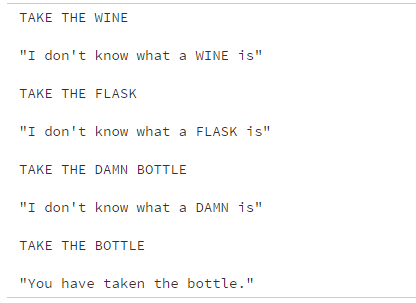
\includegraphics{images/dialogue.png}
\caption{Beispieldialog bei der Text-Parsing-Methode; Quelle: Screenshot eines Auszuges aus \cite{npcs}}
\end{figure}
\begin{figure}[here]
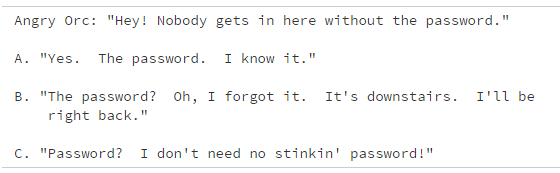
\includegraphics{images/options.png}
\caption{Beispiel für Antwortmöglichkeiten im Optionsdialog; Quelle: Screenshot eines Auszuges aus \cite{npcs}}
\end{figure}

\end{document}